\documentclass[a4paper, 11pt]{article}
\author{Kajetan Kaczmarek}
\usepackage{amsmath}
\usepackage{graphicx}
\usepackage{listings}
\usepackage[T1]{fontenc}
\usepackage[utf8]{inputenc}
\usepackage[polish]{babel}
\usepackage{color} %red, green, blue, yellow, cyan, magenta, black, white
\definecolor{mygreen}{RGB}{28,172,0} % color values Red, Green, Blue
\definecolor{mylilas}{RGB}{170,55,241}
\graphicspath{ {./} }


\lstset{language=Matlab,%
    basicstyle=\tiny,
    breaklines=true,%
    morekeywords={matlab2tikz},
    keywordstyle=\color{blue},%
    morekeywords=[2]{1}, keywordstyle=[2]{\color{black}},
    identifierstyle=\color{black},%
    stringstyle=\color{mylilas},
    commentstyle=\color{mygreen},%
    showstringspaces=false,%without this there will be a symbol in the places where there is a space
    numbers=left,%
    numberstyle={\tiny \color{black}},% size of the numbers
    numbersep=9pt, % this defines how far the numbers are from the text
    emph=[1]{for,end,break},emphstyle=[1]\color{red}, %some words to emphasise
    %emph=[2]{word1,word2}, emphstyle=[2]{style},    
}

\begin{document}
\title{Sprawozdanie STP \\* Projekt nr.1 \\* 
Zadanie 21 \\*}
\maketitle

\begin{enumerate}
\item Wyznaczanie transmitancji dyskretnej G(z) \\*
Najpierw dokonałem rozkładu na ułamki proste używając programu

\lstinputlisting{STP_P_1.m}

Otrzymane rozłożona transmitancja ma postać \[ G(s) = \dfrac{0.5893}{s-4} + \dfrac{0.5357}{s+3} +\dfrac{-0.125}{s+2} \]
Z kolei transmitancję dyskretną otrzymamy używając wzoru \[G(z) = (\dfrac{z-1}{z})Z(\dfrac{G(s)}{s}) \] Czyli dla naszej transmitancji
 \[G(z) = (\dfrac{z-1}{z})Z(0.5893\dfrac{-4}{s(s - 4)} + 0.5357\dfrac{3}{s(s + 3)} - 0.125\dfrac{2}{s(s + 2)} ) \] 
 
 Po uproszczeniu , dla T = 0.25s
  \[G(z) = 0.5893\dfrac{1-e}{z - e} + 0.5357\dfrac{1-e^{-0.75}}{z - e^{-0.75}} - 0.125\dfrac{1-e^{-0.5}}{z - e^{-0.5}}  \] 
  Czyli
  \[G(z) = \dfrac{0.779114z^2 - 0.30963236942z - 0.11275337808 }{z^3 - 3.79718 z^2 + 3.21925 z - 0.778801} \]\\
  \\
Zera układu
\begin{enumerate}
\item Dla transmitancji ciągłej \[ s_1 = -0.5 , s_2 = -1.5 \]
\item Dla transmitancji dyskretnej \[ z_1 = -0.230483 , z_2 = 0.627899\]
\end{enumerate}
Bieguny układu

\begin{enumerate}
\item Dla transmitancji ciągłej \[ s_1 = 4 , s_2 = -2 , s_3 = -3\]
\item Dla transmitancji dyskretnej \[ z_1 = 0.472367 , z_2 = 0.606531 , z_3 = 2.71828\]
\end{enumerate}
\item Reprezentacja modelu w przestrzeni stanów
Po przemnożeniu naszej transmitancji dyskretnej przez \( z^{-n} = z^{-3}\)
otrzymujemy
  \[G(z) = \dfrac{0.779114z^{-1} - 0.30963236942z^{-2} - 0.11275337808z^{-3} }{1 - 3.79718 z^{-1} + 3.21925 z^{-2} - 0.778801z^{-3}} \]
  Czyli macierze dla wariantu pierwszego wyglądają następująco
 \[ A = 	
 \begin{bmatrix}
   3.79718 & -3.21925 & 0.778801\\
   1 & 0 & 0\\
   0 & 1 & 0
  \end{bmatrix}
\]

\[C = 
\begin{bmatrix}
	0.779114 & 0.30963236942 & 0.11275337808 \\
\end{bmatrix}
\]
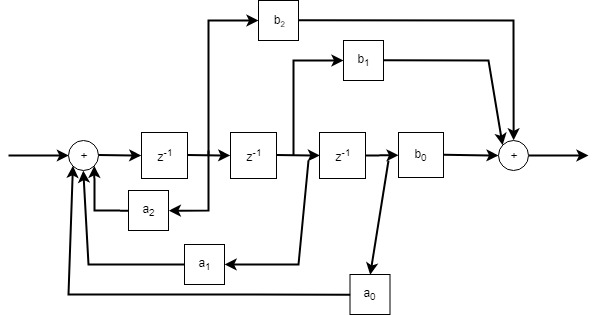
\includegraphics[width=\textwidth]{Wariant1.jpg}

Oraz dla wartiantu drugiego 

 \[ A = 	
 \begin{bmatrix}
   3.79718 & 1 & 0 \\
   -3.21925 & 0 & 1\\
   0.778801 & 0 & 0
  \end{bmatrix}
\]

\[B = 
\begin{bmatrix}
	0.779114 \\
	0.30963236942 \\
	 0.11275337808 \\
\end{bmatrix}
\]
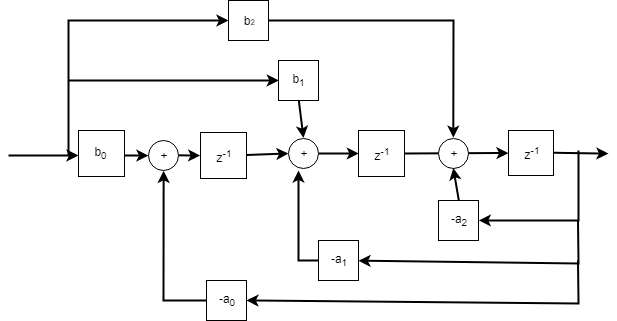
\includegraphics[width=\textwidth]{Wariant2.png}
\item Wykazanie że obie reprezentacje modelu w przestrzeni stanów można sprowadzić do tej samej transmitancji
\end{enumerate}
\end{document}
